21. $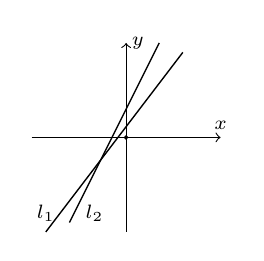
\begin{tikzpicture}[scale=0.6]
\tikzset {line01/.style={line width =0.5pt}}
\tikzset{line02/.style={line width =1pt}}
\tikzset{line03/.style={dashed,line width =0.9pt}}
\filldraw [black] (0,0) circle (1pt);
\draw [->] (-2,0) -- (2,0);
\draw [->] (0,-2) -- (0,2);
\draw[line01] (-1.7,-2) -- (1.2,1.8);
\draw[line01] (-1.2,-1.8) -- (0.7,2);
\draw (-1.7,-1.6) node {\scriptsize $l_1$};
\draw (-0.67,-1.6) node {\scriptsize $l_2$};
\draw (2,0.25) node {\scriptsize $x$};
\draw (0.25,2) node {\scriptsize $y$};
\end{tikzpicture}$ На рисунке прямая $l_1$ задана уравнением $y=k_1x+b_1,$ а прямая $l_2$ уравнением $y=k_2x+b_2.$ Сравните $k_1b_1$ и $k_2b_2.$\\
